\documentclass[14pt]{extbook} % Edit this line to change the documentclass.
% Add custom preamble content below.
% Example commands for using the Polyglossia package with French are
% included for reference.
% You may also have to edit config/lang.yml to sync up the HTML/EPUB/MOBI.
% \usepackage{polyglossia}
% \setdefaultlanguage{french}
% \DeclareTextCommandDefault{\nobreakspace}{\leavevmode\nobreak\ }

\usepackage{latex_styles/softcover}
\VerbatimFootnotes % Allows verbatim text in footnotes
\title{Padrino Book}
\subtitle{A Guide To Master The Elegant Ruby Web Framework}
\author{Matthias Günther}
\date{}

\begin{document}

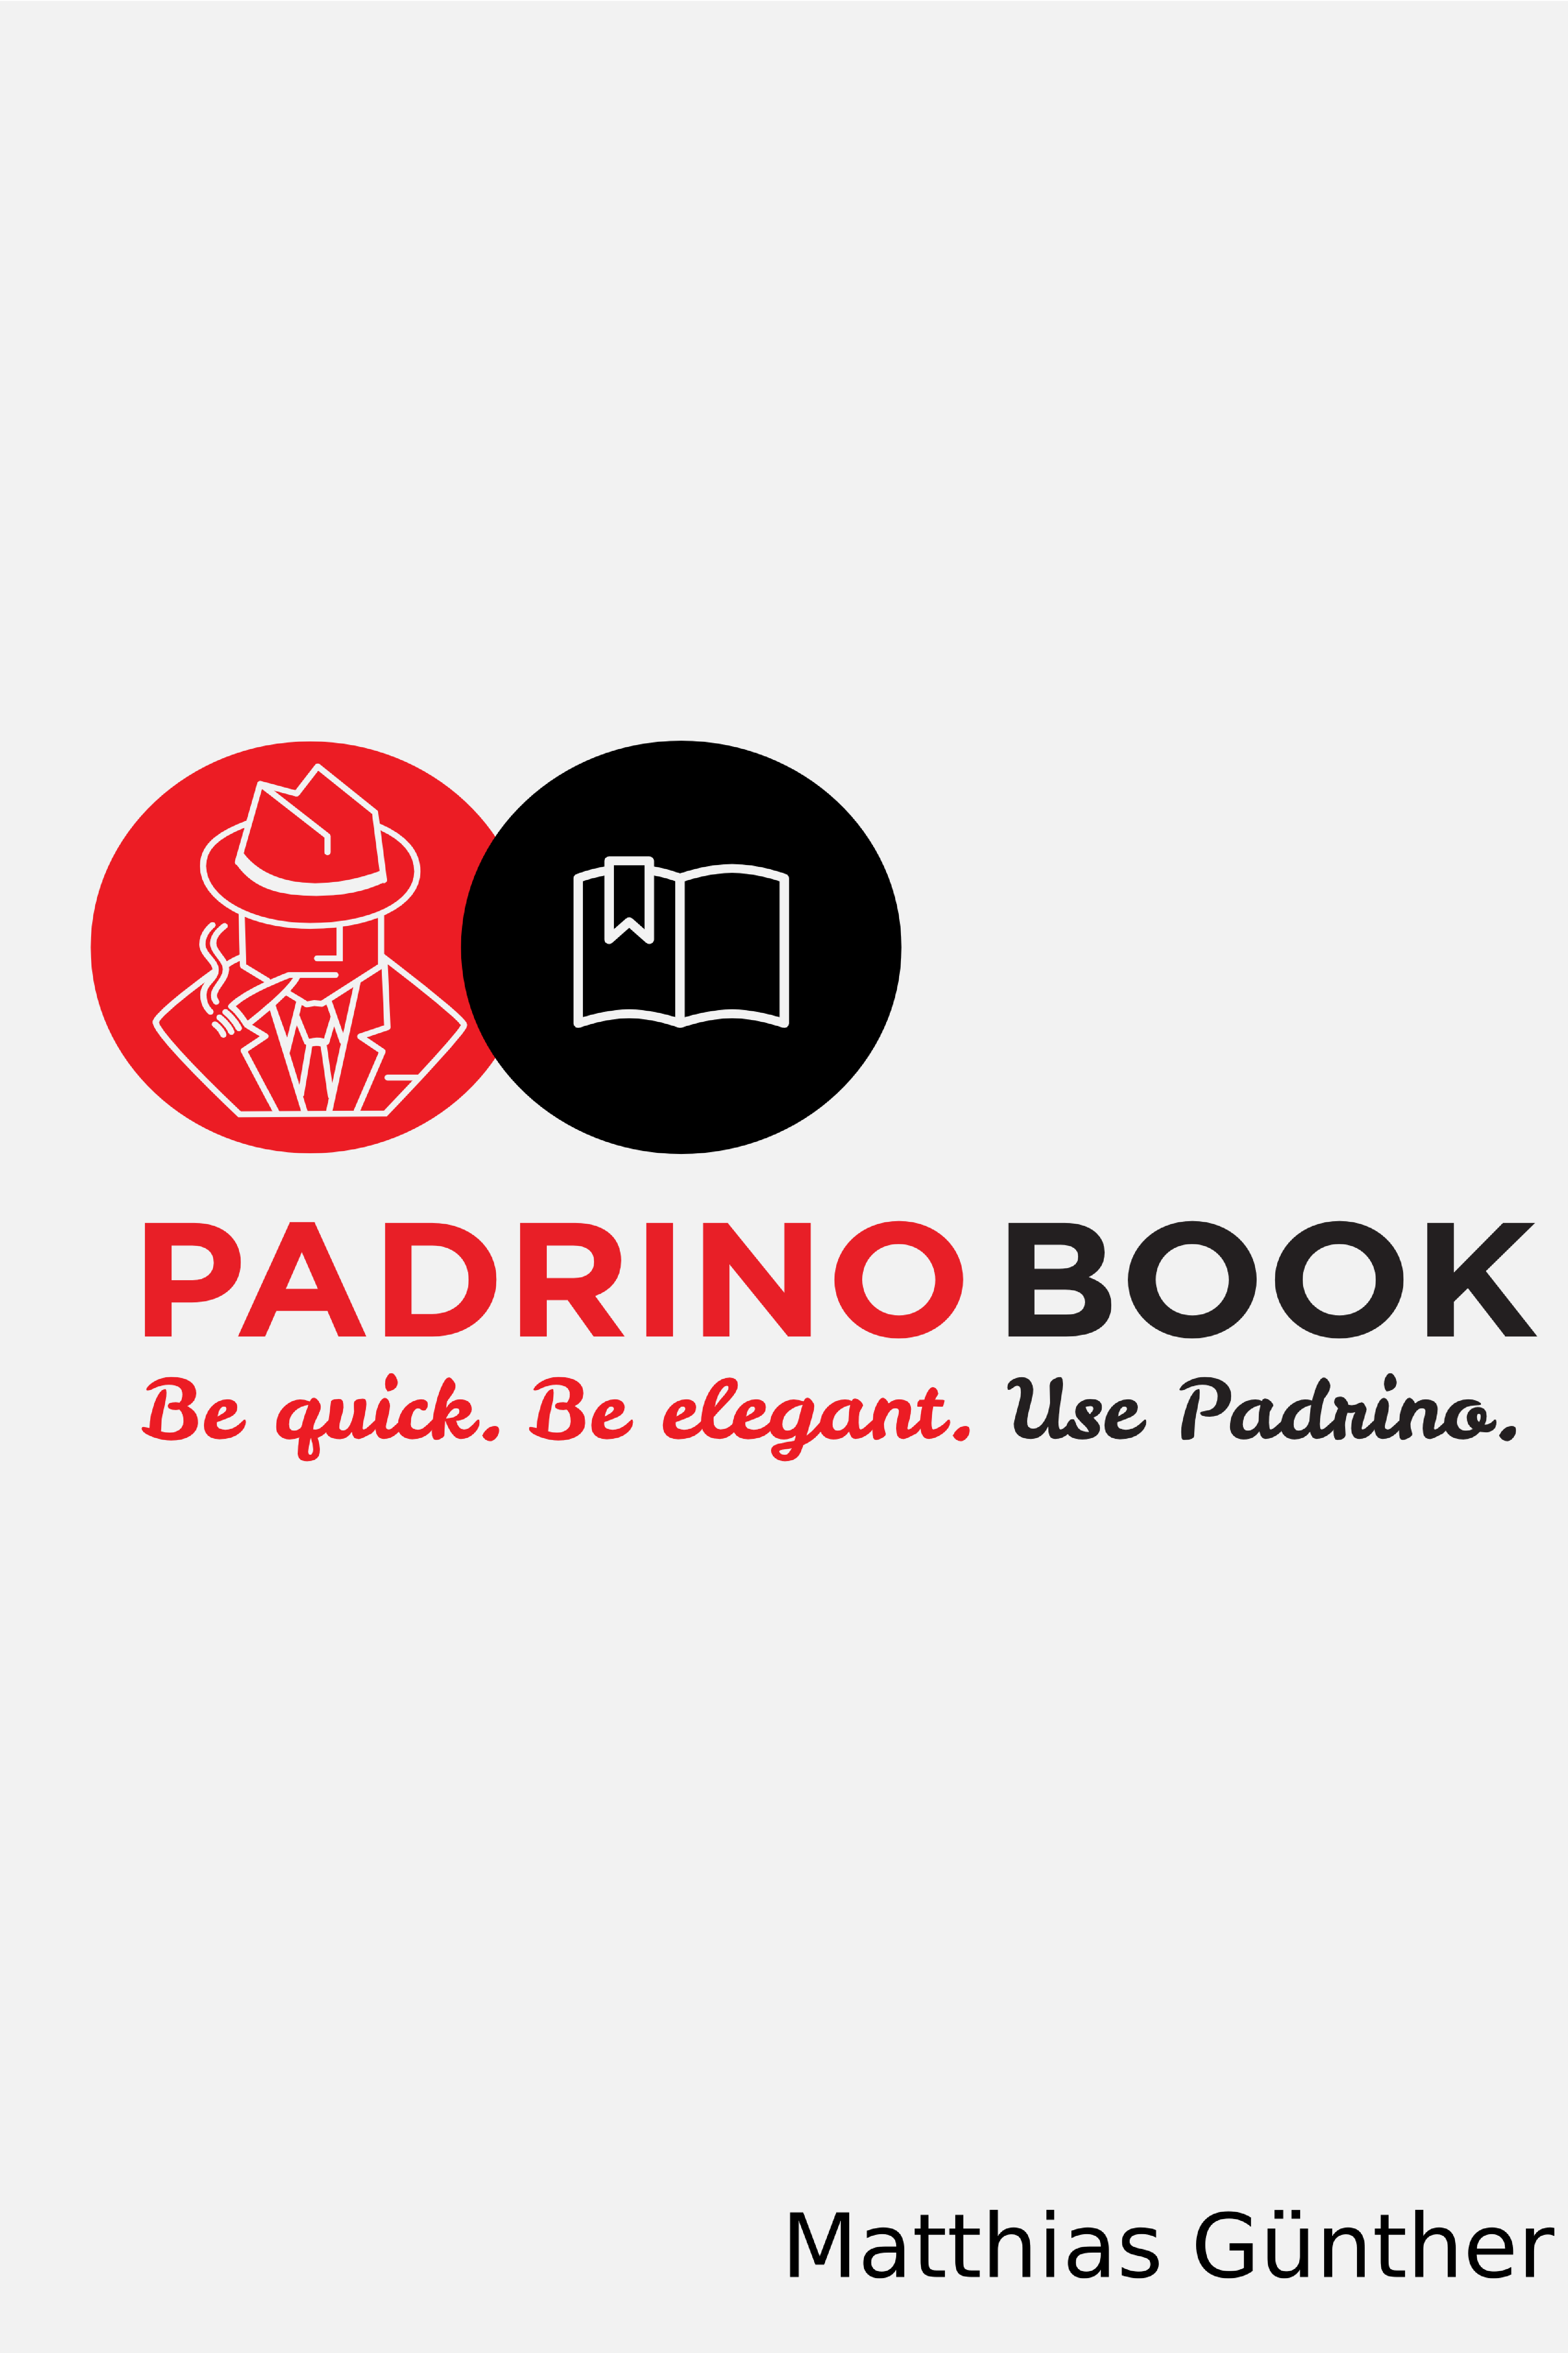
\includepdf{images/cover.pdf}
\frontmatter
\maketitle
\tableofcontents
\include{generated_polytex/preface}
\include{generated_polytex/contributors}
\mainmatter
\include{generated_polytex/01-00-introduction}
\include{generated_polytex/01-01-motivation}
\include{generated_polytex/01-02-basics-and-tools}
\include{generated_polytex/01-03-installing-ruby-with-rbenv}
\include{generated_polytex/01-04-hello-world}
\include{generated_polytex/01-05-conclusion}
\include{generated_polytex/02-00-job-vacancy-application}
\include{generated_polytex/02-01-creating-a-new-application}
\include{generated_polytex/02-02-creation-of-models}
\include{generated_polytex/02-03-user-login-and-registration}
\include{generated_polytex/02-04-user-profile}
\end{document}
